\chapter{总体概述}
%======================================================================================
% 本节描述影响产品和产品需求的一般因素。由以下4个部分构成。 
% 有一点需说明的是本节不描述具体的需求,只是使那些将要描述的具体需求更易于理解。
%======================================================================================
\section{软件概述}

	\subsection{项目介绍}
	%======================================================================================
	% 描述本软件需求所描述的项目的背景。
	% 例如:本项目是一系列版本中的一个,或者是替代某个已经存在的系统,还是一个新的独立的项目。
	%======================================================================================
	本项目是一个新的独立的项目,旨在为现代高校和企业工作团队提供一个完整高效的即时通讯系统平台;
	实现通讯,管理,公告,文件的在线支持;
	使得工作团队可以随时随地交流信息,协同合作;
	方便团队的组织和事务、活动信息的发布;
	为个人资料管理和日程安排提供高效工具。

	\subsection{产品环境介绍}
	%=========================================gongnneg=============================================
	% 描述的是本产品与其它产品或项目所组成的整体环境。
	% 1.如果本产品是独立的并完全自我包含,在此说明这一点。
	% 2.如果SRS定义的产品是更大的系统或项目的组件(此种情形经常发生),那么应:
	%	A. 	描述此大系统或项目每个组件的功能,并且标识接口。
	%	B. 	确定本软件产品主要外部接口。
	%		(注意:在此部分并不进行这些接口的详细描述;对这些接口的详细描述在SRS的其它部分提供。)
    %	C. 	描述相关产品硬件和所使用的外部设备。(注意:这只是概述性描述。)
	% 通过方块图来描述大系统或项目的主要组件,互连性以及外部接口将是非常有帮助的。
	% 本部分不应提出一个具体的设计解决方案或对解决方案的具体设计约束(具体设计约束将在具体需求章节中描述)。
	% 本部分内容是产生设计约束的基础。
	%======================================================================================
	本产品是一个相对独立的的产品,可以独立运行实现绝大多数核心功能需求,
	扩展性功能进一步支持邮箱管理,需要的其他组件是邮箱组件,包括登录认证,接收邮件和发送邮件
	功能接口,不需要其他外部设备。
\newpage
\section{软件功能}
\begin{itemize}
	\item 一对一即时通讯功能:用户可以和其他人一对一进行即时通讯。
	\item 多情境群聊功能:提供多种群聊情境,每种情境有相应的功能需求。
	\item 活动/任务发布与管理功能:在群聊中或Board上发布的任务、活动信息可以加入个人日程。
	\item 音视频通话(会议)功能:可以进行一对一或多人即时音视频通话。
	\item 通讯录功能:每个用户可以有自己的通讯录。
	\item 聊天记录功能:系统可以维护用户的聊天记录。
	\item 消息提醒功能:系统可以提示用户新的信息。
	\item Board(广场)功能:用户可以发布日志并阅读别的用户发表的日志。
	\item 个性化好友推荐功能:系统可以为用户推荐好友人选。
	\item 在线文档协作平台功能:用户可以在线共同编辑文档。
	\item 账号保护和隐私保护功能:系统可以保护用户信息。
	\item 日历管理功能:用户可以管理自己的日历。
	\item 个人本地和云端文件管理功能:用户可以通过软件管理本地或云端的文件。
	\item 邮箱接口功能:用户可以借助第三方邮箱插件管理邮箱。
\end{itemize}
软件功能描述图\ref{fig:function}
\newpage
%======================================================================================
% 概述软件的必须实现的和通过用户操作实现的主要功能。
% 这里只需要进行简要描述(例如目录列表),详细描述在详细需求部分描述。
% 对需求功能进行组织,以便于读者理解,并能指导后续的设计和测试。
% 可以用图表来表示主要需求群组之间的关系,例如:高层的数据流图,面向对象的分析等。
% 有时此部分所要求的功能概述可以从分配具体功能给此软件产品的更高层规格(如果存在的话)直接引用。
% 本节不应描述具体需求。但本节内容是具体需求章节的基础。
%======================================================================================
\begin{figure}[ht]
	\centering
	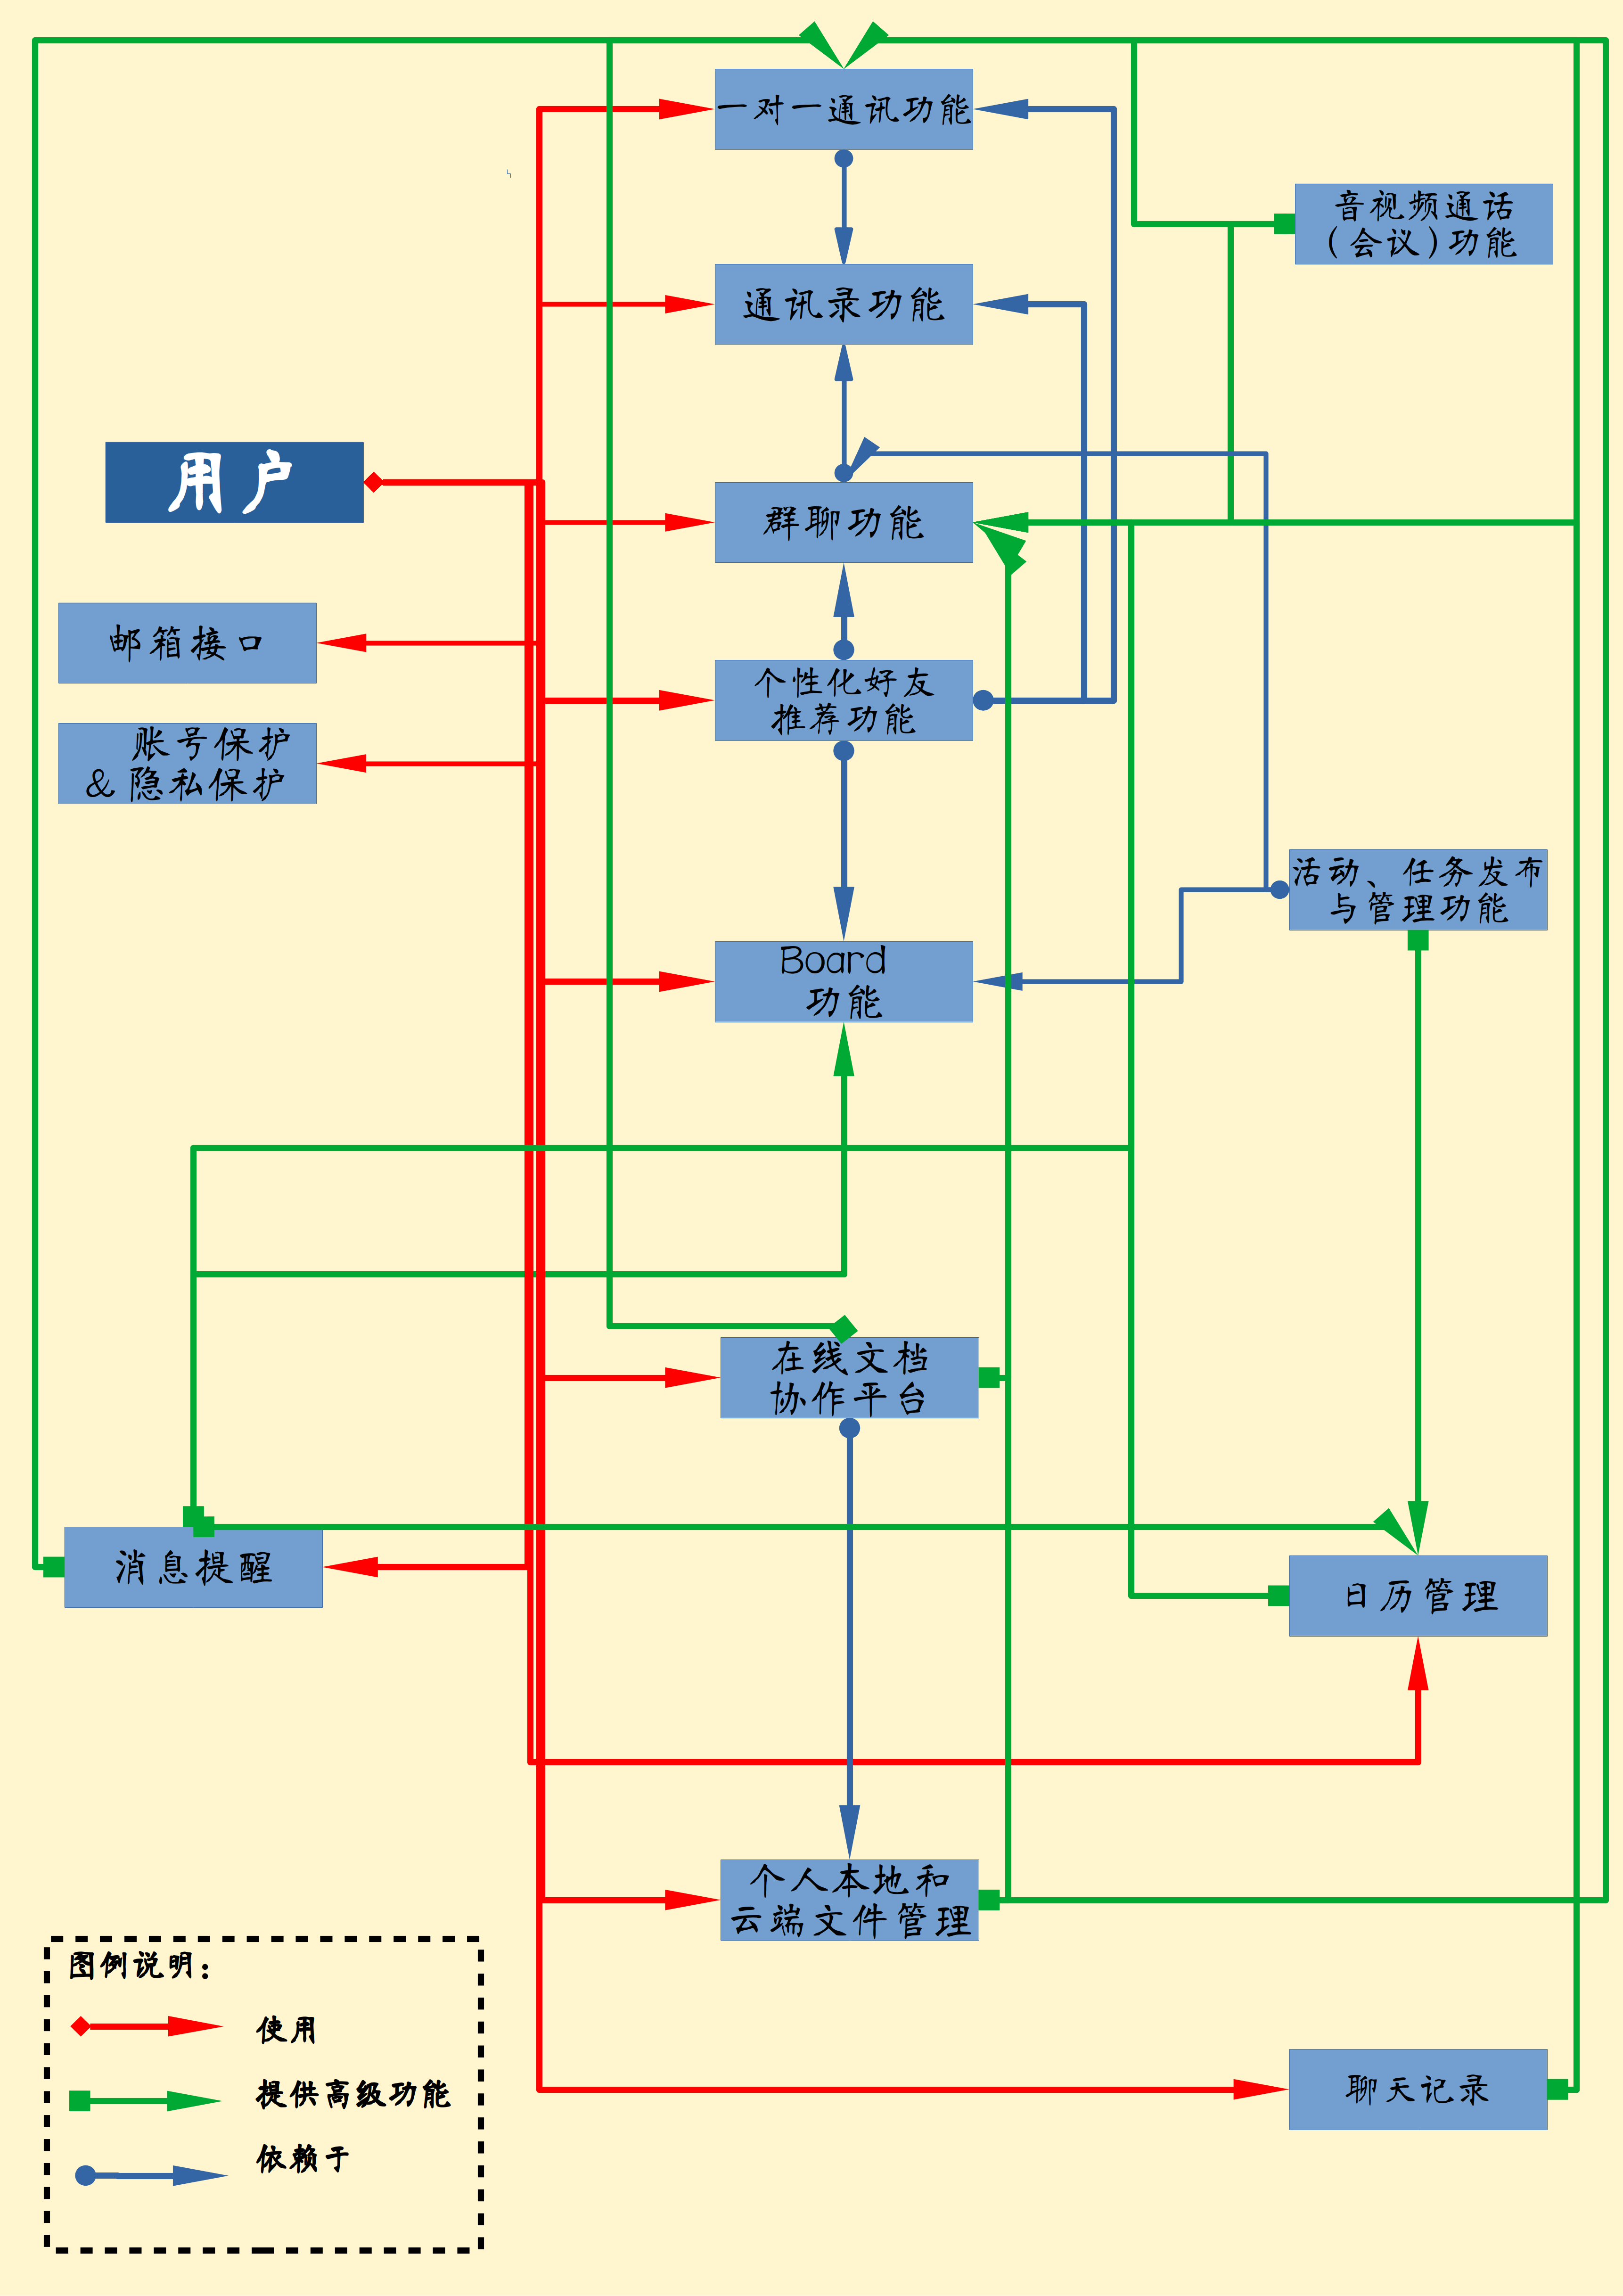
\includegraphics[scale = 0.7]{chat.png}\label{tab:classification}
	\caption{软件功能描述图}\label{fig:function}
	\note{本图片说明了即时通讯软件功能交互与依赖关系}
\end{figure}
\newpage
\section{用户特征}
%======================================================================================
% 列出对用户或系统操作者的要求,如:经验,能力,角色等。
% 本节不应描述具体需求。但本节内容是具体需求章节的基础。
%======================================================================================
\noindent
	本软件的主要目标人群包括:
	\begin{itemize}
		\item 高校大学生
		\item 科研机构研究人员
		\item 企业部门人员
		\item 工程开发团队人员
	\end{itemize}
	它主要适用于具有如下特点的人员:
	\begin{itemize}
		\item 在短期稳定的组织,如班级,实验室,团队
		\item 组织需要合作或者布置任务
		\item 需要合作编辑文档
		\item 需要频繁的信息沟通
		\item 定期开会
		\item 通信环境中有很多文件需要交换,发布、处理
		\item 有一些任务需要按时完成
		\item 日程安排严谨
		\item 对于所在环境(校园,公司)有社交需求
		\item 需要一定的通讯信息安全保证
		\item 有频繁、重要的邮件需要处理
	\end{itemize}
	针对以上用户特点,本软件可以高效,专业、全面地提供即时通讯及配套的各种功能。
\section{假设和依赖关系}
%======================================================================================
% 列出可能影响SRS中需求的所有的假设因素(与已知事实相对而言),
% 包括准备使用的第三方或商业组件,操作和开发环境的问题约束等。
% 如果上述假设不正确、没有被告知或者改变了都将对项目产生影响。
% 列出项目对外部条件的依赖,例如重用其他项目的模块等。
% 如果在其他文档(例如项目计划或范围文档等)里已经描述了,在这里可以不用描述。
%======================================================================================
\begin{itemize}                                                      
	\item 操作平台:Android,IOS,Windows,Linux
	\item 内部依赖关系:\\
		一对一通讯系统功能依赖于通讯录功能\\
		群聊功能依赖于通讯录功能\\
		个性化好友推荐功能依赖于一对一通讯功能、群聊功能、通讯录功能和Board功能\\
		在线文档协作平台依赖于个人文件和云端文件管理功能\\
		活动、任务发布与管理功能依赖于群聊功能和Board功能
	\item 外部依赖关系:\\
		邮箱接口功能依赖于外部邮箱组件
	\item 服务器端:借助第三方服务器
\end{itemize}